\documentclass[]{article}

%Deutsche Bezeichnungen für angezeigte Namen (z.B. Innhaltsverzeichnis etc.)
\usepackage[ngerman]{babel}

% prints dummy text
\usepackage{blindtext}

% Ränder bei Bedarf zeigen
%\usepackage{showframe}

%Erlaubt unteranderem Umbrücke captions
\usepackage{caption}

%Kompakte Listen
\usepackage{paralist}

%Zitate besser formatieren und darstellen
\usepackage{epigraph}

%Zeilenabstand 1,5
\usepackage[onehalfspacing]{setspace}

%Verbesserte Darstellung der Buchstaben zueinander
\usepackage[stretch=10]{microtype}

%Unterstützung von Umlauten und anderen Sonderzeichen (UTF-8)
\usepackage{lmodern}
\usepackage[utf8]{luainputenc}
\usepackage[T1]{fontenc}

%Einfachere Zitate
\usepackage{epigraph}

%Verwendung von Akronymen
\usepackage[printonlyused]{acronym}

%Unterstützung der H positionierung (keine automatische Verschiebung eingefügter Elemente)
\usepackage{float} 

%Erlaubt Umbrüche innerhalb von Tabellen
\usepackage{tabularx}

%Erlaubt Seitenumbrüche mit Tabellen
\usepackage{longtable}

%Erlaubt die Darstellung von Sourcecode mit Highlighting
\usepackage[outputdir=out]{minted}

%Definierung eigener Farben bei nutzung eines selbst vergebene Namens
\usepackage[table,xcdraw]{xcolor}

%Vektorgrafiken
\usepackage{tikz}

%Grafiken (wie jpg, png, etc.)
\usepackage{graphicx}

%Grafiken von Text umlaufen lassen
\usepackage{wrapfig}

%Ermöglicht Verknüpfungen innerhalb des Dokumentes (e.g. for PDF), Links werden durch "hidelink" nicht explizit hervorgehoben
\usepackage[hidelinks, ngerman]{hyperref}

%Einbindung und Verwaltung von Literaturverzeichnissen
\usepackage{csquotes} %wird von biber benötigt
\usepackage[style=alphabetic, backend=biber, bibencoding=utf8]{biblatex}
\addbibresource{references/references.bib}

% for enumeration
\usepackage{enumitem}

%-------------------------------Zusätzliche Anpassungen und Modifikationen--------------------------------------------%
%Pluszeichen in der Referenz beim zitieren ausblenden
\renewcommand*{\labelalphaothers}{}

\addto{\captionsngerman}{\renewcommand{\abstractname}{Abstract}}

%Exposé Type
\newcommand*{\exposeType}[1]{\gdef\@exposeType{#1}}

%%Exposé Type (CHOOSE ONE)
\exposeType{Bachelorabschlussarbeit}
%\exposeType{Masterabschlussarbeit}
%\exposeType{Forschungsprojekt A}
%\exposeType{Forschungsprojekt B}

\title{\bf Exposé - \@exposeType:\protect\\ Untersuchungen von Style Transfer Methoden für die Verwendung mit leistungsarmer Hardware}
\author{Christoph Stach}
\date{07.01.2019}

\begin{document}

\maketitle

\begin{otherlanguage}{ngerman}
	\begin{abstract}
		Die Abschlussarbeit im Bereich der Angewandte Informatik handelt darum verschiedene Style Transfer Methoden zu implementieren,
		die Konzepte zu verstehen und Sie auf Tauglichkeit für Systeme mit leistungsarmer Hardware zu testen. Style Transfer ist ein Bereich des 
		Deep Learning. Es werden dabei zwei, oder mehrere, willkürliche Bilder zu einem neuen Bild kombiniert. Beim ersten Bild wird der Inhalt aus
		dem Bild herausgefiltert, z.B. aus einem Foto auf dem ein Vogel zu sehen ist. Aus dem zweiten Bild wird der Stil herausgefiltert, 
		z.B. aus einem abstrakt gezeichneten Gemälde. Das Ergebnis ist die Mischung aus Objekt und Style. Die Ausrichtung, ob das Ergebnis mehr 
		Objekt oder eher Style ist, kann durch Parameter beeinflusst werden. Es sollen unterschiedliche Algorithmen untersucht werden und
		die Ergebnisse miteinander veglichen werden.
	\end{abstract}
\end{otherlanguage}

\pagebreak

\section{Motivation}
Style Transfer ist ein intressantes Forschungsobjekt. Es müssen 

\section{Zielsetzung}
Ziel des Projektes ist ein Softwaresystem zu erstellen das in der Lage ist
Style Transfer auf Geräten mit leistungsarmer Hardware zu ermöglichen. Dabei sollen Mechanismen des Style Transfer
untersucht werden und sukzessiv verbessert werden.

\section{Vorgehen}
Nach der Einarbeitung in die Grundlagen von Style Transfer \cite{DBLP:journals/corr/GatysEB15a} \cite{DBLP:journals/corr/JohnsonAL16} Methoden,
müssen entsprechende Algorithmen gefunden werden. Da es sich um die Manipulation von Bildern handelt, werden Convolutional Neural Networks
\cite{lecun-gradientbased-learning-applied-1998} zum Einsatz kommen, die sich dazu eignen Features aus Bildern zu extrahieren. 
Im nächsten Schritt muss ein Datensatz wie Image Net \cite{imagenet_cvpr09} benutzt oder in entsprechender Größe generiert werden, mit dem ein solches Netzwerk trainiert 
werden kann. Auch möglich ist der Einsatz von Transfer Learning mit bereits bestehenden, vortrainierten Netzwerkarchitekturen
\cite{DBLP:journals/corr/SimonyanZ14a}, um die Ergebnisse zu verbessern. Letztendlich muss das Netzwerk auf den verwendeten Datensatz durch
Backpropagation \cite{doi:10.1162/neco.1989.1.4.541} optimiert werden.
\\
Die Implementierung des Models in den Prototypen eines Softwaresystems soll der Veranschaulichung der Ergebnisse dienen.

\pagebreak

\section{Erfordernisse und Randbedingungen}
Da das Berechnen von Deep Neural Networks und Convolutional Neural Networks sehr rechenintensiv sein kann,
werden diese normalerweise auf Serversystemen mit eingebauter Graphic Processing Unit trainiert und ausgeführt. Das soll bei der Evaluation der 
Modelle berücksichtigt werden, damit Ergebnisse in einem vertretbaren Zeitaufwand auf Systemen ohne GPU zu berechnen sind.

\section{Zeitplan}
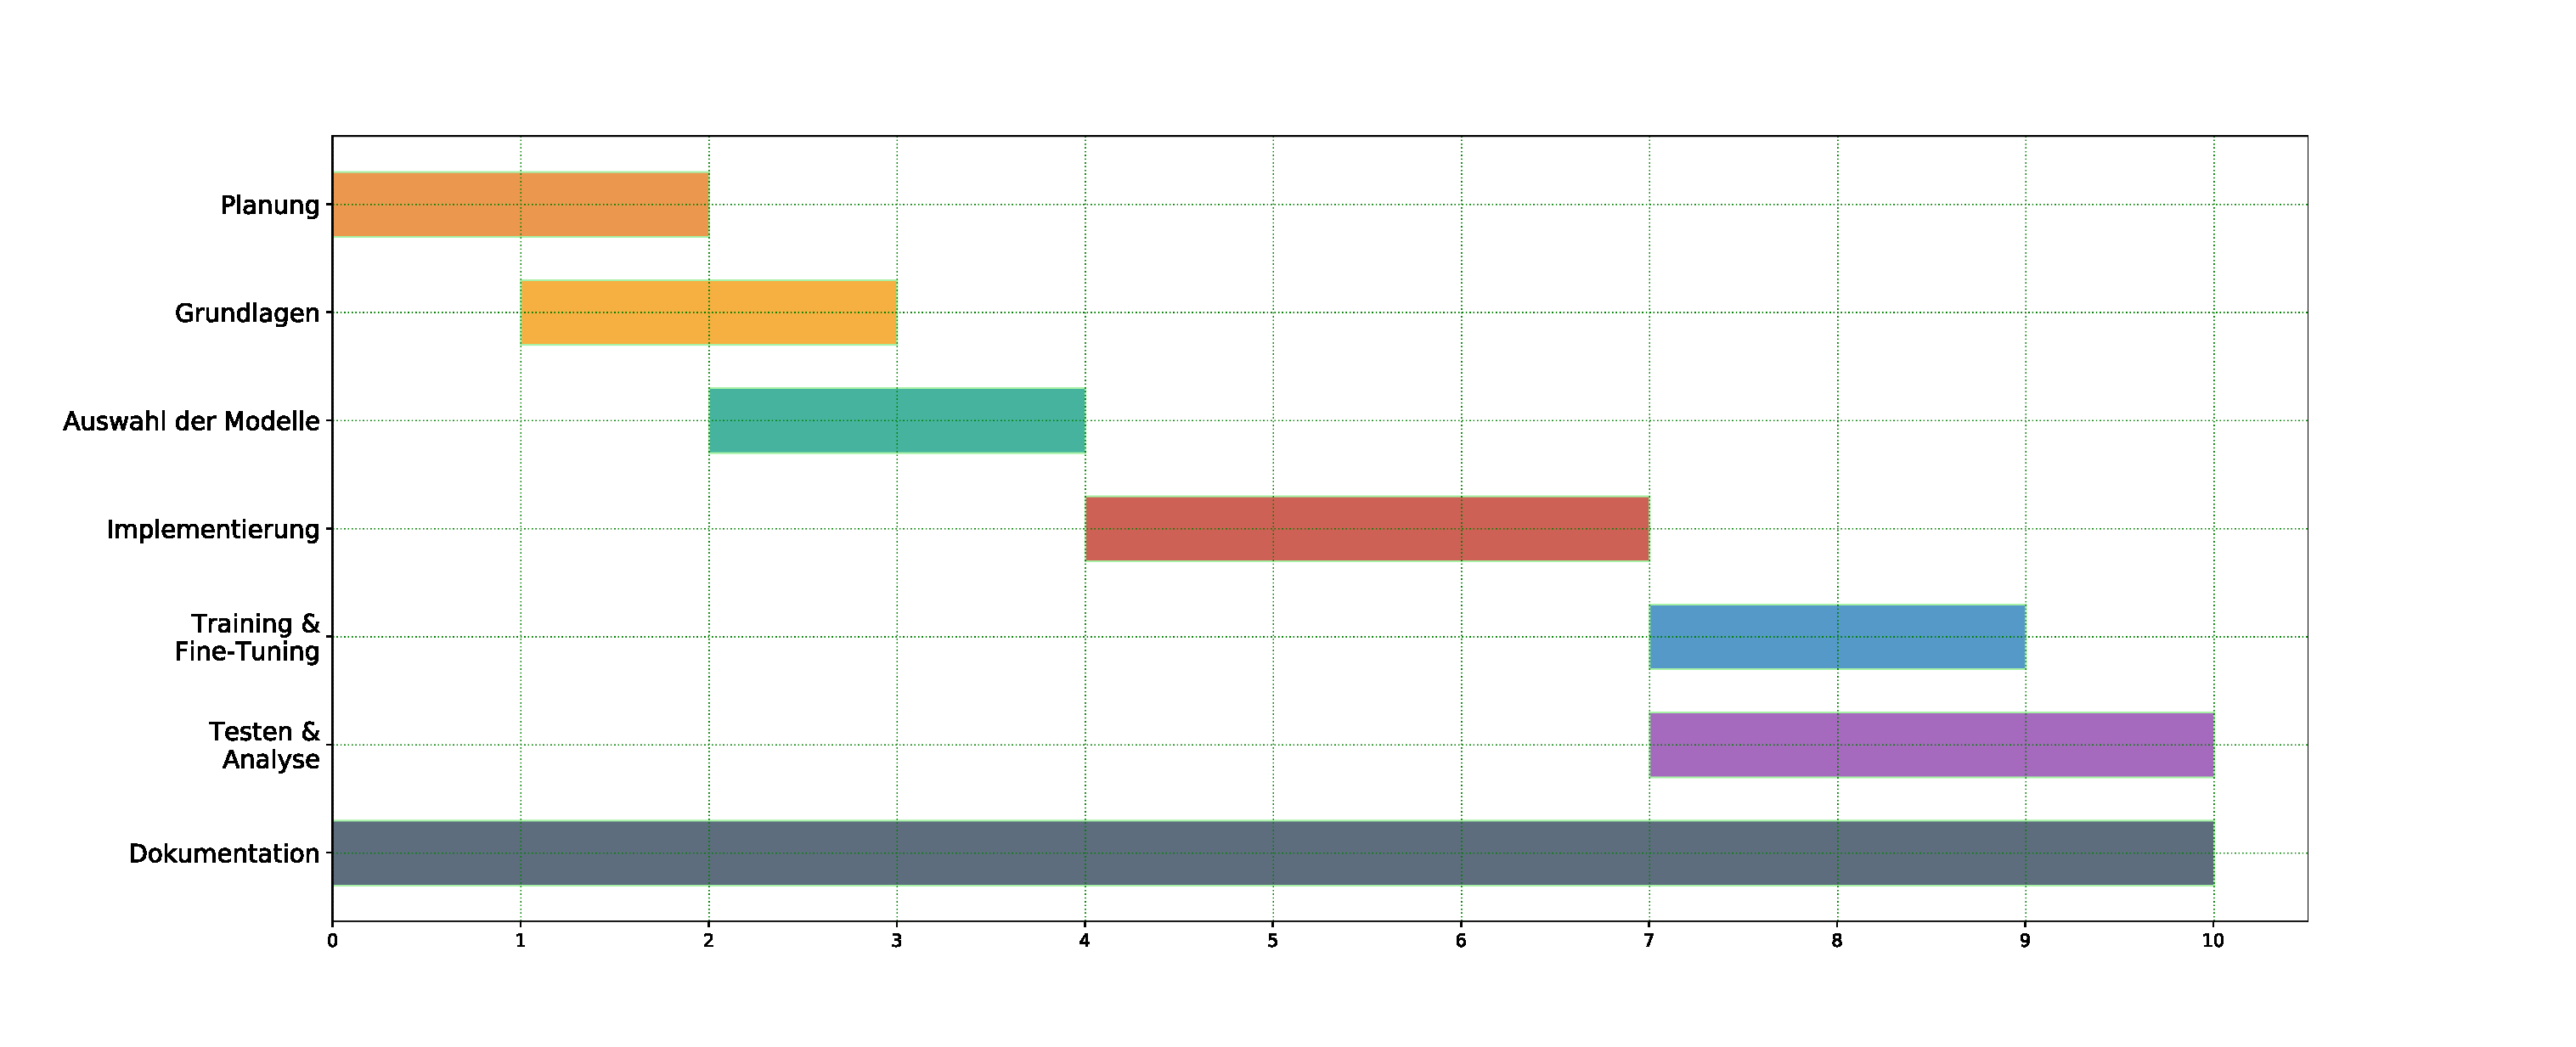
\includegraphics[width=1.00\textwidth]{resources/gantt.eps}
Das Gantt-Diagramm stellt den vorläufigen Zeitplan des Projektes da.
Dieser kann sich jedoch während des Projektverlaufes noch ändern und wird bei Bedarf angepasst.
Besonders zu beachten ist, dass das Training eines Neural Networks in Verbindung mit großen Datenmengen viel Zeit in Anspruch nehmen kann.
Deswegen wurden für das Training vorläufig zwei Wochen veranschlagt.

\section{Erwartete Ergebnisse}
Das Ergebnis des Projektes ist der lauffähige Prototyp eines Softwaresystems mit der dazugehörigen Dokumentation und Erklärung
aller verwendeten Algorithmen und Modelle. Der Prototyp soll eine Verschmischen von einem Style mit einem Bild ermöglichen. 
Sollte das erfolgreich implementiert werden können, soll er erweitert werden um die Möglichkeit mehrere verschiedene Styles zu wählen.
Ziel ist es außerdem den performantesten Ansatz des Algorithmus in den Prototypen zu implementieren.

\pagebreak

\section{Vorläufige Gliederung}

\begin{enumerate}
	\item Zusammenfassung (Abstract)
	\item Einleitung
	\item Grundlagen
	\item Analyse
	\item Konzeption
	\begin{enumerate}[label*=\arabic*.]
		\item Suche und Auswahl geeigneter Modelle
		\item Implementierung einer Basisversion der Modelle
		\item Verbesserungen und Erweiterungen an Modellen
		\item Hyperparameter-Tuning und Training
		\item Implementierung der Modelle in den Prototypen eines Softwaresystems
	\end{enumerate}
	\item Implementierung
	\item Test
	\item Evaluation
	\item Fazit / Ausblick
\end{enumerate}

\pagebreak

\defbibfilter{scientific}{
	type=article or
	type=inbook or
	type=book or
	type=unpublished or
	type=inproceedings or
	type=incollection or
	type=manual or
	type=phdthesis
}

\printbibliography[heading=bibintoc, filter=scientific, title={Literaturangaben}]

\end{document}
